\section{Graphen und Netzwerke}
\begin{tabularx}{\textwidth}{p{4cm} X}
  Exakter Algorithmus
    & Findet optimale Lösung\\
  Heuristik
    & Findet gute, aber normalerweise nicht optimale Lösung\\
  Greedy Algorithmus
    & Trifft zu jedem Zeitpunkt aktuell beste Wahl, d.h. lokales Optimum; müssen nicht zu globalen Optimum führen \\
  Ungerichteter Graph
    & Graph mit endlicher Menge Ecken $V$ und Kanten $v,w \in E$\\
  Einfacher Graph
    & Keine Schlingen, keine parallelen Kanten \\
  Schlinge
    & Kante, wo Anfang- gleich Endecke ist ($vv$)\\
  Pfad 
    & Folge von Ecken $v_0, v_1, ... v_k$\\
  Kreis 
    & Pfad, wo die Anfangsecke gleich der Endecke: $v_0 = v_k$\\
  Azyklischer Graph, Wald
    & Graph, der keinen Kreis enthält\\
  Baum
    & Azyklischer, zusammenhängender Graph\\
  Bipartiter Graph
    & Die Ecken können in zwei Teilmengen aufgeteilt werden, so dass jede Kante je eine Ecke in beiden Teilmengen hat \skript{10}\\
  Eulerkreis
    & Kreis, der jede Kante des Graphen genau ein Mal enthält\\
  Hamiltonkreis
    & Kreis, der alle Ecken genau ein Mal besucht und zudem in der Startecke startet und endet\\
  Euler-/Hamiltongraph
    & Wenn Graph einen Euler- oder Hamiltonkreis enthält\\
\end{tabularx}


\subsection{Repräsentation von Graphen \skript{3}}
  
\begin{center}
	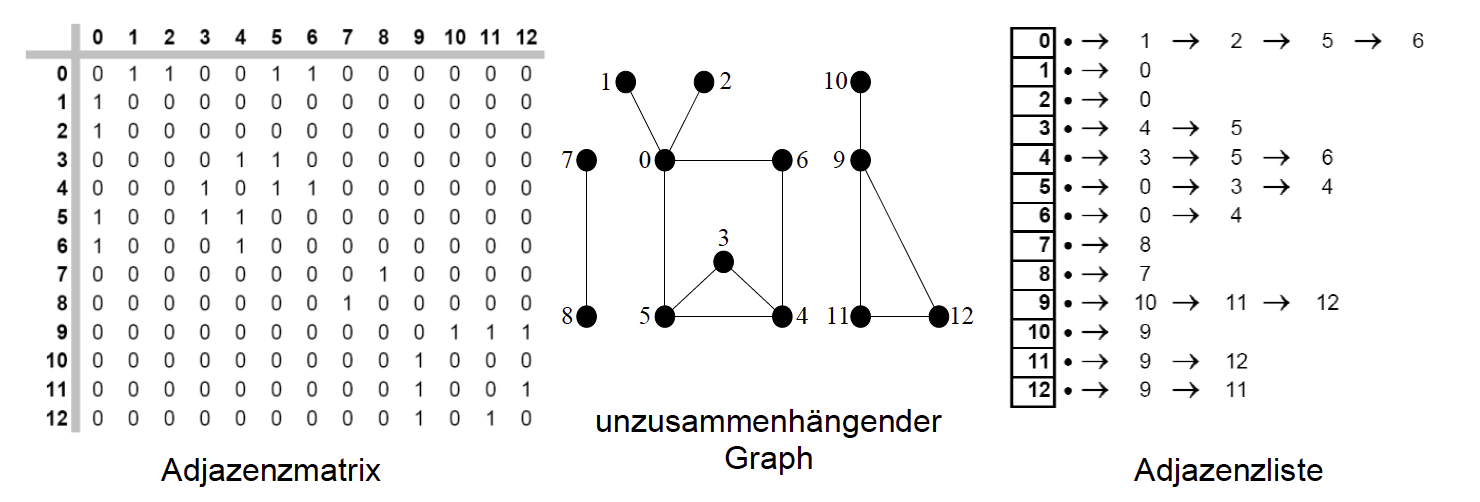
\includegraphics[width=0.8\textwidth]{Content/Graphen/AdjListMatrix.png}
	  
	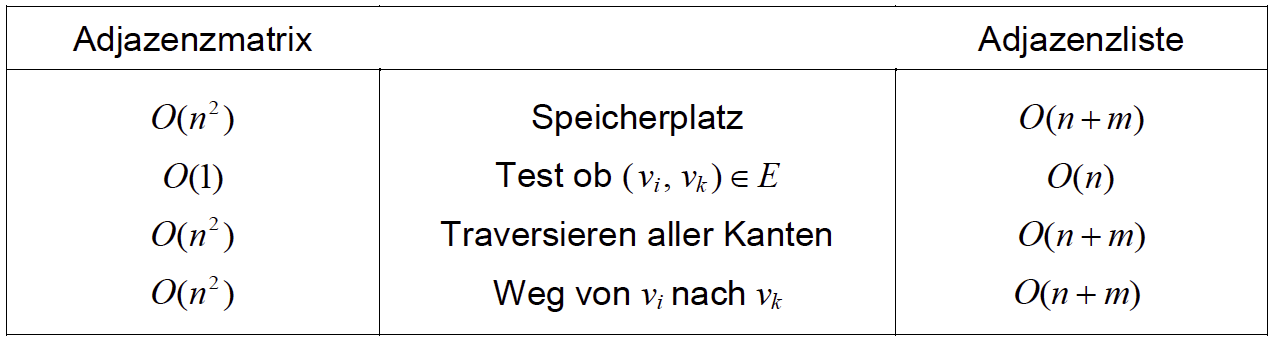
\includegraphics[width=0.5\textwidth]{Content/Graphen/KomplAdj.png}
\end{center}


\subsection{Entscheidungsbaum-Verfahren \skript{4}}
	Das Travelling-Salesman-Problem (\skript{31}), wo jede Stadt genau ein Mal besucht werden darf, ist lösbar mit dem Branch-And-Bound Verfahren.


\subsection{Traversieren von Graphen \skript{9}}

\begin{minipage}{0.5\textwidth}
	\subsubsection{Tiefensuche (Depth-First Search, DFS)}
		Ausgehend von einer Ecke, wird immer weiter zur nächsten Ecke durch den Baum "traversiert", bis das Ende erreicht ist. Dann wird von der nächsten unbesuchten Ecke weitertraversiert, bis alle Ecken besucht sind. Dies ist eine Last-In-First-Out (LIFO) Strategie.
		
		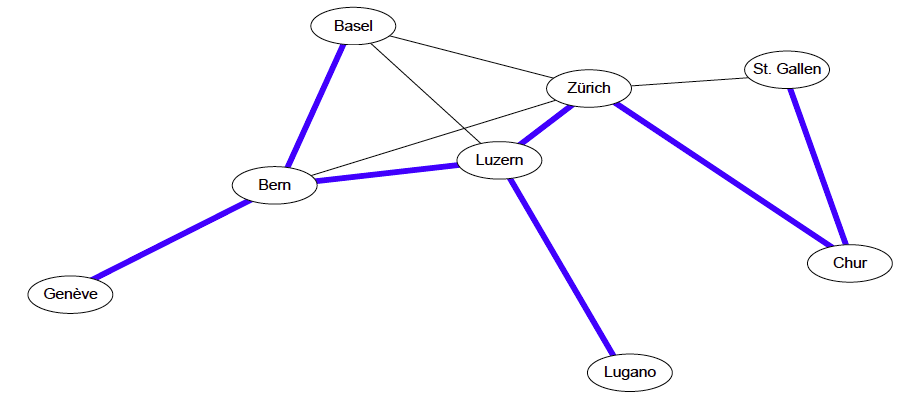
\includegraphics[width=\textwidth]{Content/Graphen/DFS.png}
		\begin{center}
		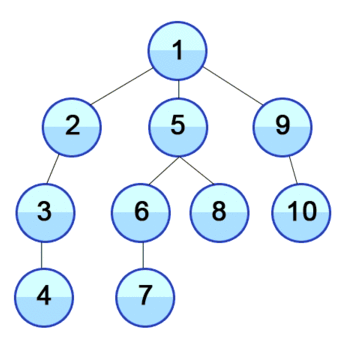
\includegraphics[width=0.3\textwidth]{Content/Graphen/tiefensuche.png}\\
		Output: 4,3,2,7,6,8,5,10,9,1\end{center}
\end{minipage}
\begin{minipage}{0.5\textwidth}
	\subsubsection{Breitensuche (Breadth-First Search, BFS)}
	  	Von einer Ecke werden alle benachbarten Ecken aufgesucht und im nächsten Schritt einer dieser benachbarten Ecken besucht. Dies ist eine First-In-First-Out (FIFO) Strategie.
	  	
	  	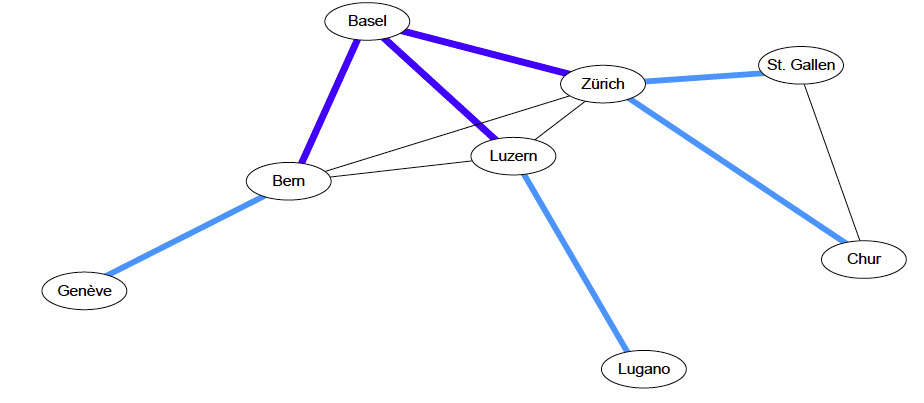
\includegraphics[width=\textwidth]{Content/Graphen/BFS.png}  
	  	\begin{center}
	  	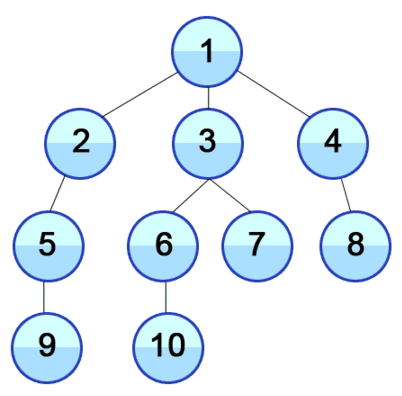
\includegraphics[width=0.3\textwidth]{Content/Graphen/breitensuche.png}\\
	  	Output: 1,2,3,4,5,6,7,8,9,10
	  	\end{center}
\end{minipage}

	
% MSTs
\subsection{Minimum Spanning Tree (MST)}

MST = Aufstellen eines Minimalen Baums: Summe aller Kantengewichte ist minimal unter allen verbundenen Knoten.
	
	\begin{tabularx}{\textwidth}{p{4cm} X p{4cm}}
	  \textbf{Prim}-Algorithmus
	    & Läuft über Ecken, ist greedy
	    & $O(n^2)$ \\
	  \textbf{Kruskal}-Algorithmus
	    & Läuft über Kanten, ist greedy
	    & $O(m \log(m))$\\
	  \textbf{MST-Heuristik} zur Lö\-sung des TSP
	    & Von bestehendem MST aus, wird in beliebige Richtung iteriert
	    & $O(n)$ ??
	\end{tabularx}


\subsubsection{Prim-Algorithmus}
Setzt Ecken ($O(n^2)$) Zwischengraph ist immer zusammenhängend.
\begin{enumerate}
	\item Beliebige Startecke $v_0$ für den MST wählen
	\item Ecke $v_i$ mit kleinstem Abstand zu einer Ecke im MST hinzufügen
	\item Punkt 2 wiederholen bis alle Ecken im MST
\end{enumerate}


\subsubsection{Kruskal-Algorithmus}
Setzt Kanten ($O(m \log(m))$) Zwischengraph ist allenfalls unzusammenhängend.
\begin{enumerate}
	\item Kante mit kleinstem Gewicht in den MST aufnehmen
	\item Kante $e_i$ mit kleinstem Gewicht, die zwei Ecken verbindet die noch nicht durch den MST verbunden sind, im MST aufnehmen
	\item zu 2 bis alle Ecken verbunden sind
\end{enumerate}


\subsubsection{MST-Heuristik zur Lösung des TSP}
Generiert Hamiltonkreis (Lösung des TSP) aus MST (Lösung muss nicht optimal sein!, Lösung ist abhängig vom Startpunkt)

\begin{enumerate}
	\item Jede Kante im MST verdoppeln (Eulergraphen)
	\item Eulerkreis auswählen (durchläuft alle Kanten)
	\item Eulerkreis durchlaufen und dabei alle bereits besuchten Knoten überspringen (Hamiltonkreis)
\end{enumerate}


% Minimaler Weg
\subsection{Minimaler Weg}

\subsubsection{Probleme}
    \begin{tabular}{ll}
      Source-sink shortest path
        & Kürzesten Weg zwischen einer Ecke (Quelle/source) und einer andern Ecke (Senke/sink) \\
      Single source shortest paths
        & Kürzeste Wege von einer Ecke (Quelle/source) zu allen anderen Ecken \\
      All pairs shortest paths
        & Kürzeste Wege zwischen allen Eckenpaaren\\
    \end{tabular}
  \subsubsection{Algorithmen}
    \begin{tabularx}{\textwidth}{p{3cm} p{4cm} X r}
      \textbf{Algorithmus} & \textbf{Löst} & \textbf{Bemerkungen} & \textbf{Compl.} \\
      \hline
      \textbf{Dijkstra} \skript{14} 
        & Source-sink shortest path, single source shortest path
        & Kantengewichte $\omega(v_i v_j) \geq 0$; Greedy; Loop über alle bereits besuchten Ecken: Suche minimale Distanz zu nächster Ecke. Der Weg, der am Schnellsten am Ziel ist, gewinnt.
        & $O(n^2)$\\
      \hline
      \textbf{Bellman-Ford}
        & Source-sink shortest path, single source shortest path
        & Auch negative Kantengewichte möglich; n~Knoten, m~Kanten
        & $O(n\cdot m)$\\
      \hline
      \textbf{A*} 
        & Single source shortest path
        & Heuristische Methode des Dijkstra, beschleunigte Laufzeit, findet optimale Lösung, benötigt viel(!) Speicher
        & ?\\
      \hline
      \textbf{Floyd-Warshall} \skript{16}
        & All pairs shortest paths 
        & Gerichtete Kreise möglich, Kantengewichte $\omega(v_i v_j) \geq 0$
        & $O(n^3)$\\
      \hline
    \end{tabularx}
    
    
\subsubsection{Dijkstra}
Sucht die kürzeste Verbindung zwischen Knoten $v_0$ und $v_n$ Kantengewicht müssen positiv sein! (sonst kann es zu nicht-optimalen Lösungen führen, da ein nicht beachteter Umweg schlussendlich kürzer gewesen wäre)
Die Menge $V$ enthält alle Ecken die bereits erreicht wurden.
$l_i$ ist der kürzeste Weg von der Ecke $v_0$ zur Ecke $v_i$.

\begin{enumerate}
	\item Beliebige Startecke $v_0$ wählen und in die Ecken-Menge $V$ aufnehmen
	\item Aus den von $V$ direkt erreichbaren Ecken diejenige zu $V$ hinzufügen, die zu $v_0$ die kürzeste Distanz hat
	%\item Diejenige Ecke zu $V$ hinzufügen, die mit dem kleinsten Abstand $w$ (von $v_0$ aus gemessen) von einer Ecke in $V$ erreicht wird
	\item $l_j = l_i + w$ ($j$ ist die neue Ecke und $i$ die Ecke, die bereits in $V$ ist, $w$ ist die Distanz zwischen $i$ und $j$)
	\item Gehe zu 2 bis die Ecke $v_n$ zu $V$ hinzugefügt wird
\end{enumerate}

\begin{center}
	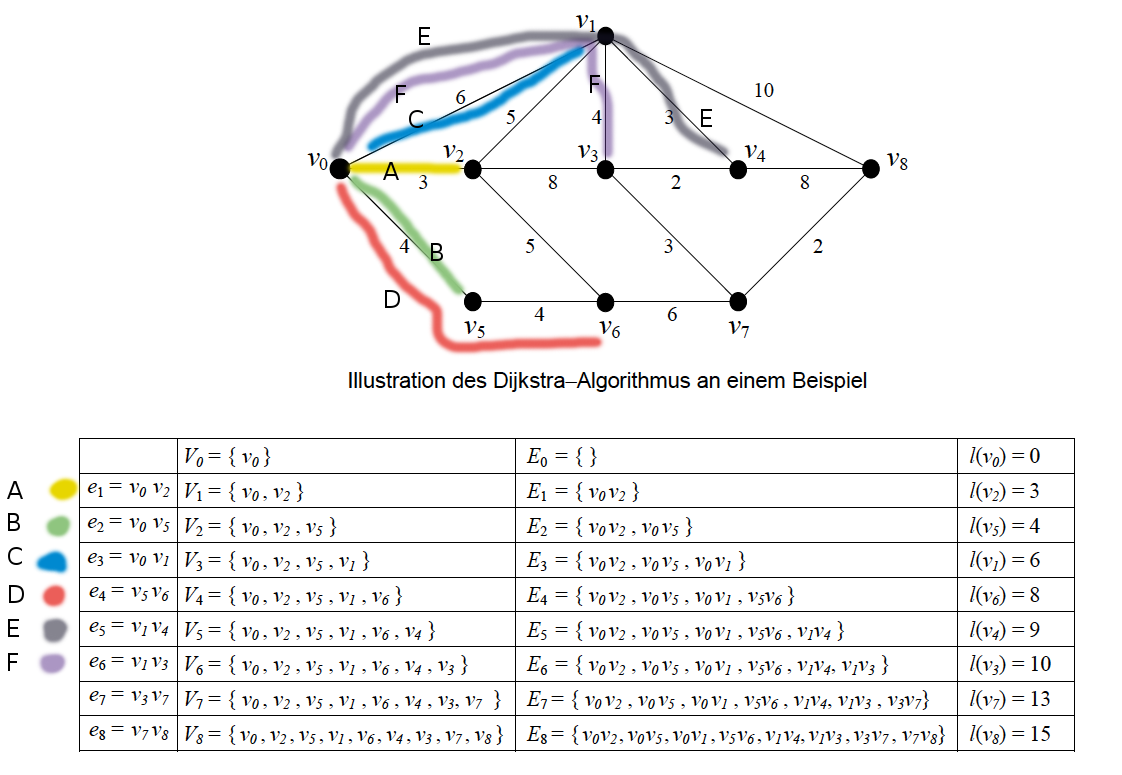
\includegraphics[width=0.8\textwidth]{Content/Graphen/Dijkstra.png}
\end{center}


\subsubsection{A*}
Der A*-Algo. untersucht immer die Koten zuerst, die wahrscheinlich schnell zum Ziel führen. Diese Wahrscheinlichkeit wird ermittelt, in dem jedem bekannten Knoten $x$ ein Wert $f(x)$ zugewiesen wird. $f(x)$ beschreibt die Distanz vom Start zum Ziel über den verwendeten Knoten ist. Der Knoten mit dem kleinsten $f(x)$ wird als nächster untersucht.
\[ f(x) = g(x) + h(x) \qquad \qquad g(x): \text{ Weg vom Startknoten bis zu }x  \qquad h(x): \text{ Weg von $x$ zum Zielknoten (Heuristik)}\]
Eine Heuristik für die Verbindung von Städten wäre z.B. die Luftlinie. Für die Durchführung des Algos wird eine \textbf{Closed-List} (untersuchte Knoten) und eine \textbf{Open-List} (gefundene, aber noch nicht untersuchte Knoten) verwendet. \textbf{Gefundene Knoten} sind, die die eine Verbindung mit einem Knoten der Closed-List haben.\\

\textbf{Bsp.:} Gesucht ist der kürzeste Weg von $Post$ nach $A$.
Bei diesem Beispiel wird für die Distanzheuristik $h(x)$ zwischen den Knoten $v_i$ und $v_j$ der Betrag $h(x)=|\textcolor{red}{i}-\textcolor{red}{j}|$ verwendet ((\textcolor{red}{rot}) $A=1$, $B=2$, etc.).

\begin{minipage}{0.5\textwidth}
	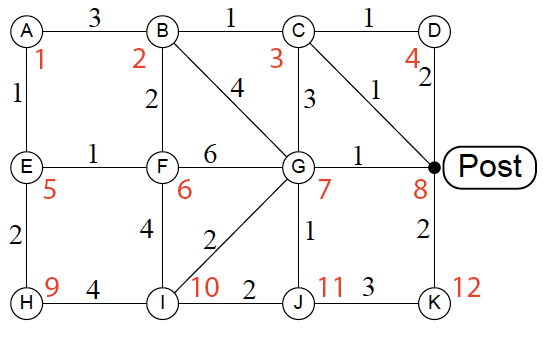
\includegraphics[width=\textwidth]{Content/Graphen/PostAStar.png}
\end{minipage}
\hfill
\begin{minipage}{0.5\textwidth}
	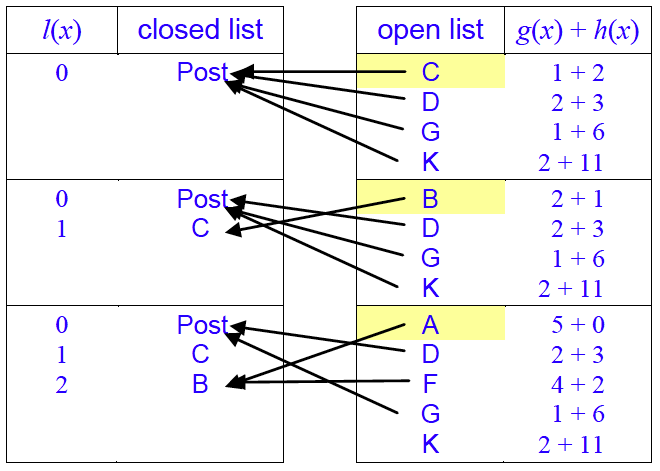
\includegraphics[width=\textwidth]{Content/Graphen/AStar.png}
\end{minipage}

Der Minimale Weg von der Post zum Knoten A beträgt 5 und kann rückwärts rekonstruiert werden:\\ $A\rightarrow B\rightarrow C \rightarrow Post$\\

\subsubsection{Floyd-Warshall}
Alle Kreise müssen ein nicht negatives Gewicht haben! Der Algorithmus ist konzipiert für gerichtete Graphen, funktioniert auch für ungerichtete (beide Richtungen gleiches Gewicht).

$shortestPath(i,j,k)$ gibt den kürzesten weg vom Knoten $v_i$ nach $v_j$, wobei der Weg über die ersten $k$ Knoten führen kann ($v_0,...,v_{k-1}$).

Die Funktion kann rekursiv implementiert werden:
\[ shortestPath(i,j,k+1) = \min \begin{cases} shortestPath(i,j,k) \qquad \qquad \qquad \qquad \qquad \text{Weg bereits bekannt (führt über $v_0, \ldots, v_{k-1}$)}\\ shortestPath(i,k,k)+shortestPath(k,j,k) \qquad  \text{Weg führt über $k$ und von dort nach $j$} \end{cases} \]

Hat ein Graph keine Kante von $v_i$ nach $v_j$ dann wird das Gewicht auf $\infty$ gesetzt!

Das Resultat des Algos ist eine Matrix, in der die kürzesten Distanzen zwischen allen Knoten angegeben ist.

\begin{enumerate}
	\item Init: setze $shortestPath(i,j,0)$ (Pfade von $v_i$ nach $v_j$ ohne Zwischenknoten)
	\item entwickle $shortestPath(i,j,k+1)$ für $k=0,1,...,n-1$ rekursive (überschreiben der Elemente bei kürzerem Weg)
	\item Matrix enthält alle kürzesten Wege
\end{enumerate}

\textbf{Bsp.:} (nichts eingetragen $=\infty$)

\begin{minipage}{0.5\textwidth}
	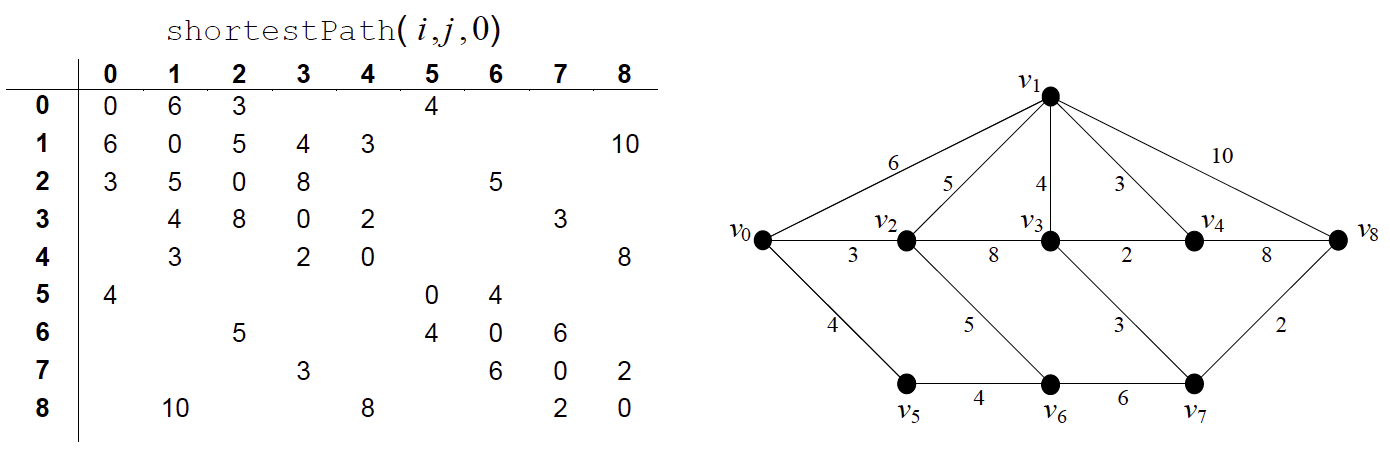
\includegraphics[width=\textwidth]{Content/Graphen/FloydWarshall1.png}
\end{minipage}
\begin{minipage}{0.5\textwidth}
	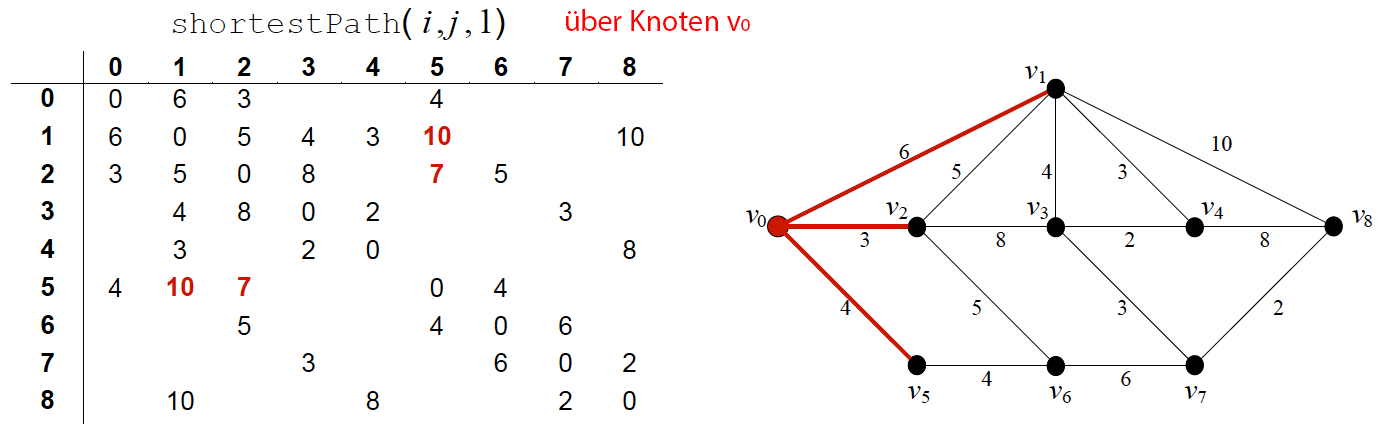
\includegraphics[width=\textwidth]{Content/Graphen/FloydWarshall2.png}
\end{minipage}
\begin{minipage}{0.5\textwidth}
	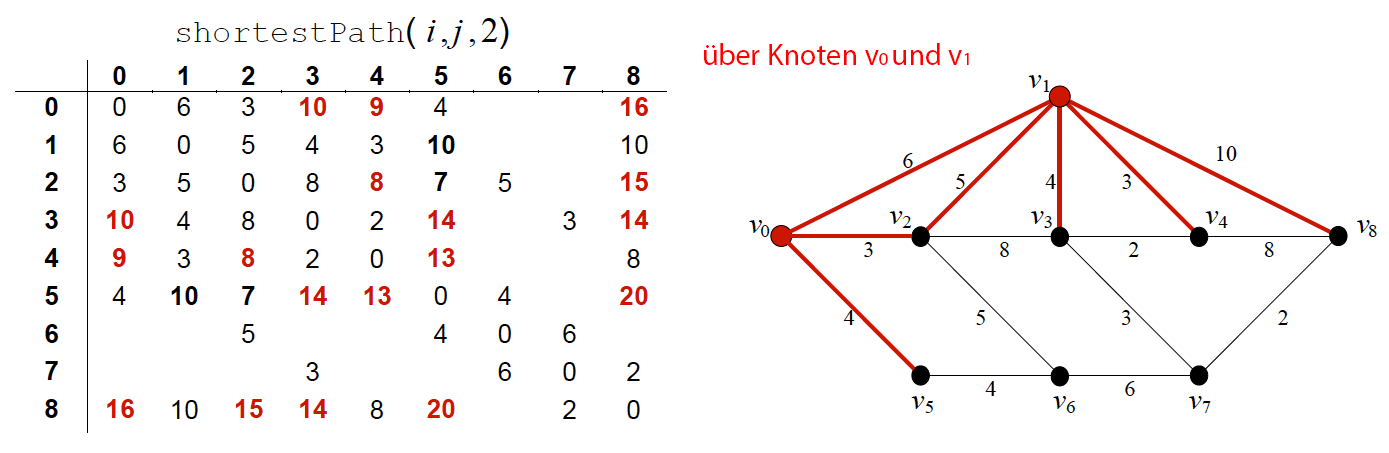
\includegraphics[width=\textwidth]{Content/Graphen/FloydWarshall3.png}
\end{minipage}
\begin{minipage}{0.5\textwidth}
	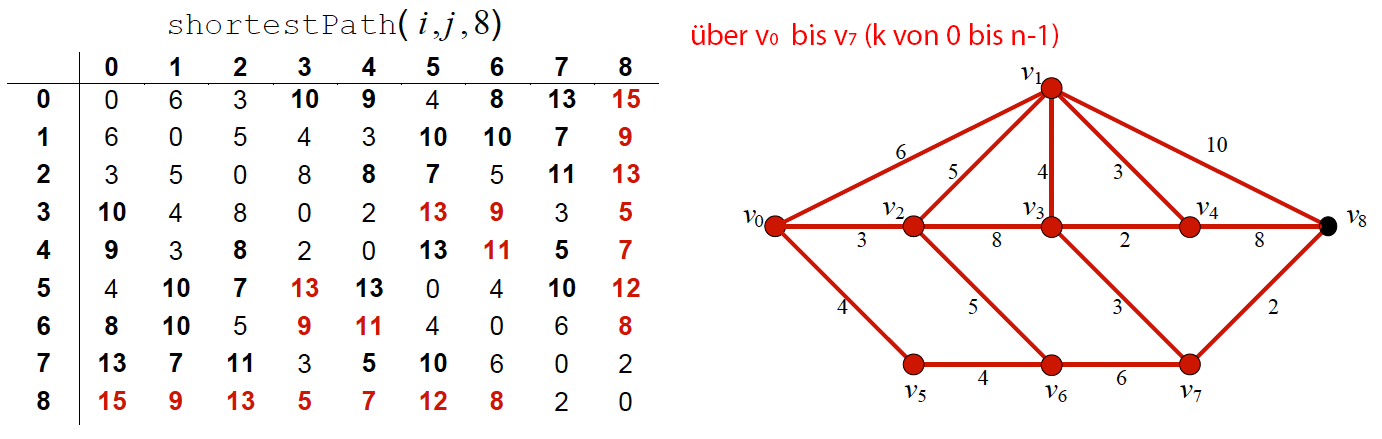
\includegraphics[width=\textwidth]{Content/Graphen/FloydWarshall4.png}
\end{minipage}

Aus der resultierenden Matrix kann nicht nur der kürzeste sondern auch der längste Pfad entnommen werden. Dieser wird auch Durchmesser des Graphen genannt.


%
% Netzwerke
%
\section{Netzwerke}
Jede Kante $vw$ hat jetzt auch eine Kapazität $c(vw)$, welche eine Obergrenze für den Fluss $f(vw)$ darstellt. Zusätzlich können den Kanten noch Kosten $k(vw)$ angefügt werden.
  
  \begin{tabularx}{\textwidth}{l X}
    Verteilungsproblem
      & Objekte von einem oder mehreren Orten (sources) an eines oder mehrere Ziele (sinks) zu verteilen\\
    Matching-Probleme
      & Zuordnung von Mengen, kann auch als bipartite Graphen interpretiert werden (bspw. Partnervermittlung) \\
    Schnitt-Probleme
      & Kanten entferne, um Netzwerk zu zerlegen (bspw. max. Anzahl Unterbrüche in Kommunikationsnetz)\\
  \end{tabularx}

% Reduktion auf Maxflow-Problem
\subsection{Reduktion auf Maxflow-Problem}

Viele bestehenden Probleme können auf Maxflow-Probleme reduziert werden.
 

\begin{minipage}{0.6\textwidth}
\textbf{Mehrere Quellen / Mehrere Senken} (Übung II.5/1):\\
	\begin{enumerate}
		\itemsep-1mm
		\item Neue Quelle $s$ einführen (Kantenkapazitäten $c_s$ entsprechen der Summe der wegführenden Kapazitäten)
		\item Neue Senke $t$ einführen (Kantenkapazitäten $c_t$ entsprechen der Summe der hinführenden Kapazitäten)
	\end{enumerate}
\end{minipage}
\begin{minipage}{0.4\textwidth}
	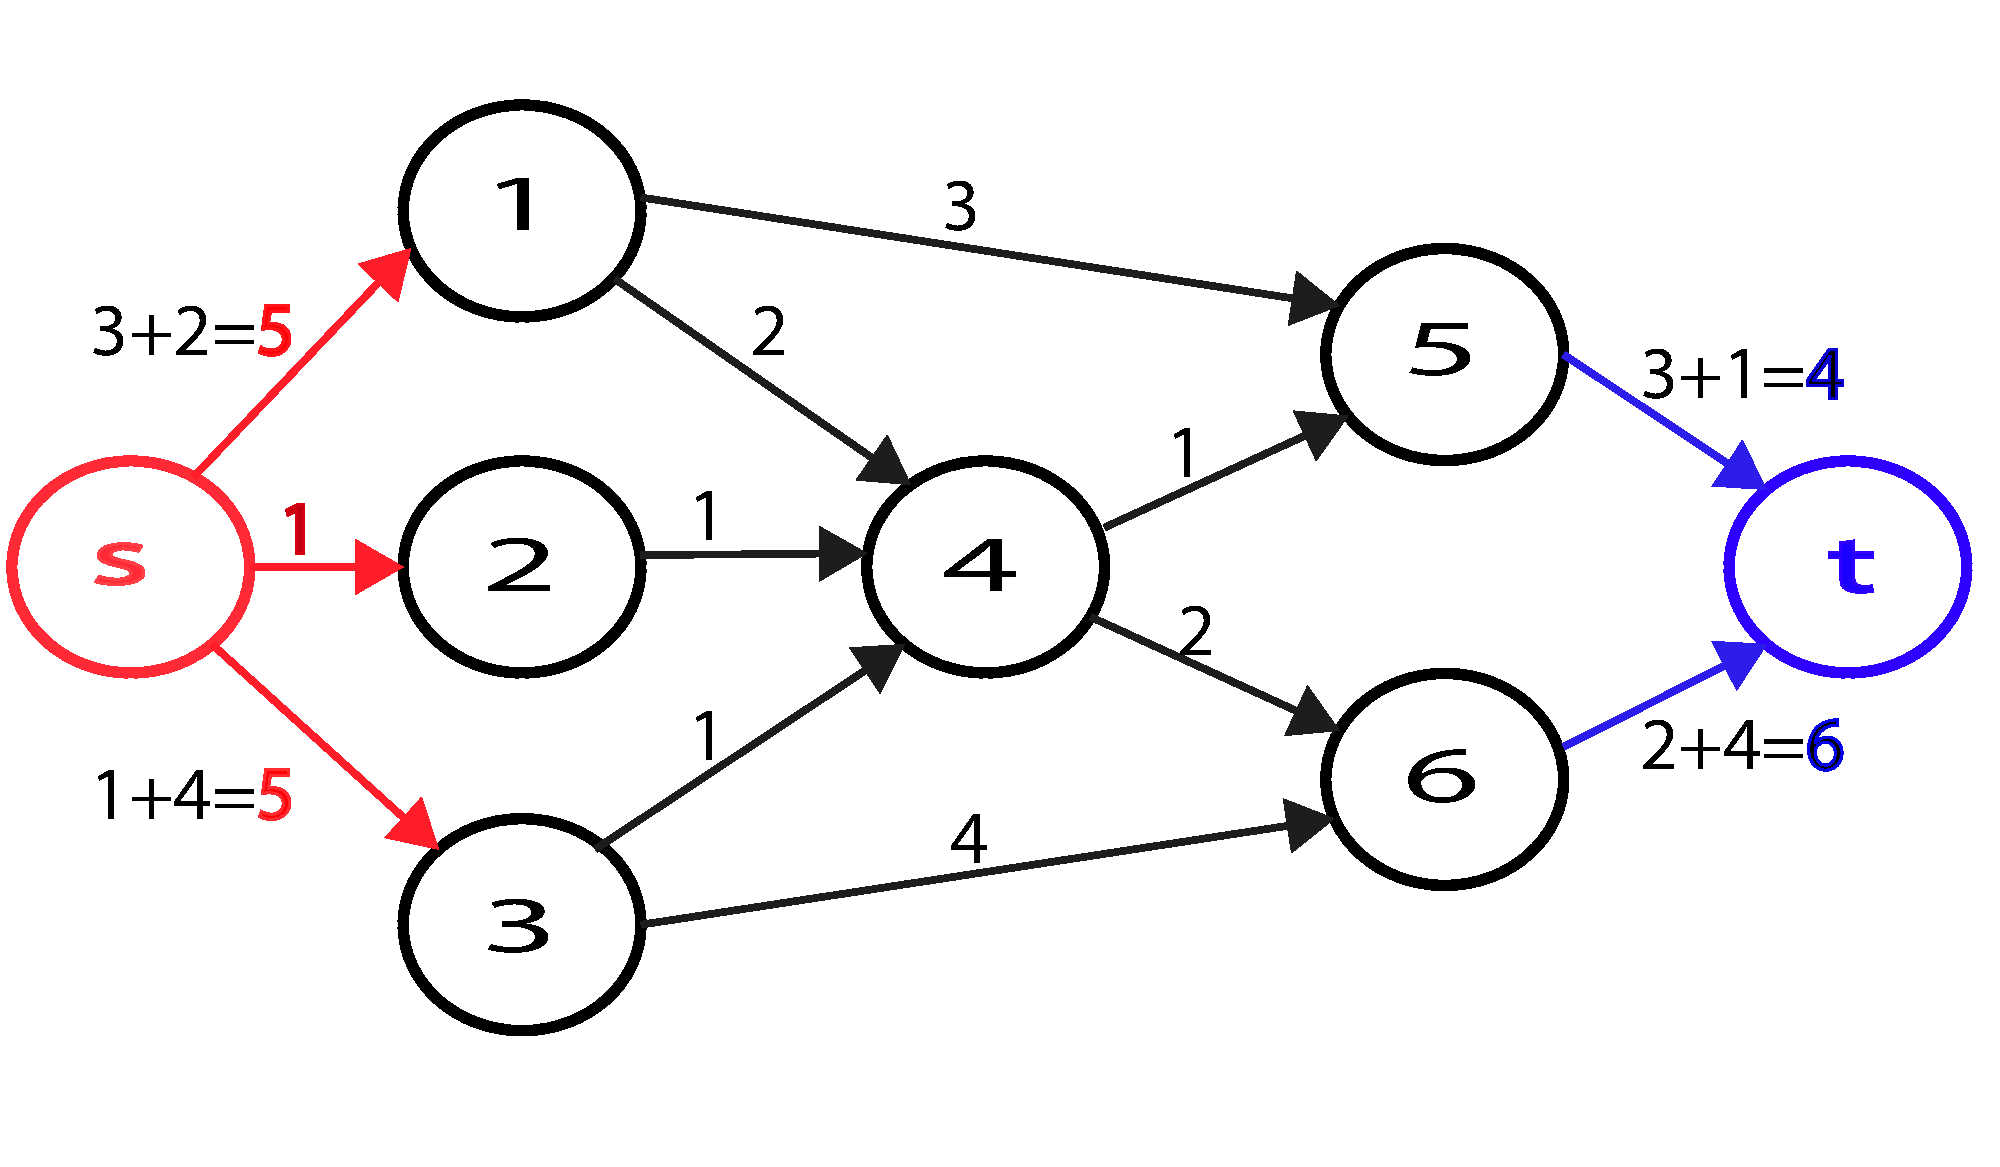
\includegraphics[width=\textwidth]{Content/Graphen/MultiSrcSink.pdf}
\end{minipage}

\textbf{Einschränkung durch Maximalkapazität:}\\
Begrenzungen durch Einführen von zusätzlichen Knoten.

\begin{minipage}{0.6\textwidth}
	\textbf{Begrenzte Output-Kapazität:}\\
	
	Neuen Knoten einführen (Kantenkapazitäten $c$ entspricht der beschränkten Output-Kapazitäten)
\end{minipage}
\begin{minipage}{0.4\textwidth}
	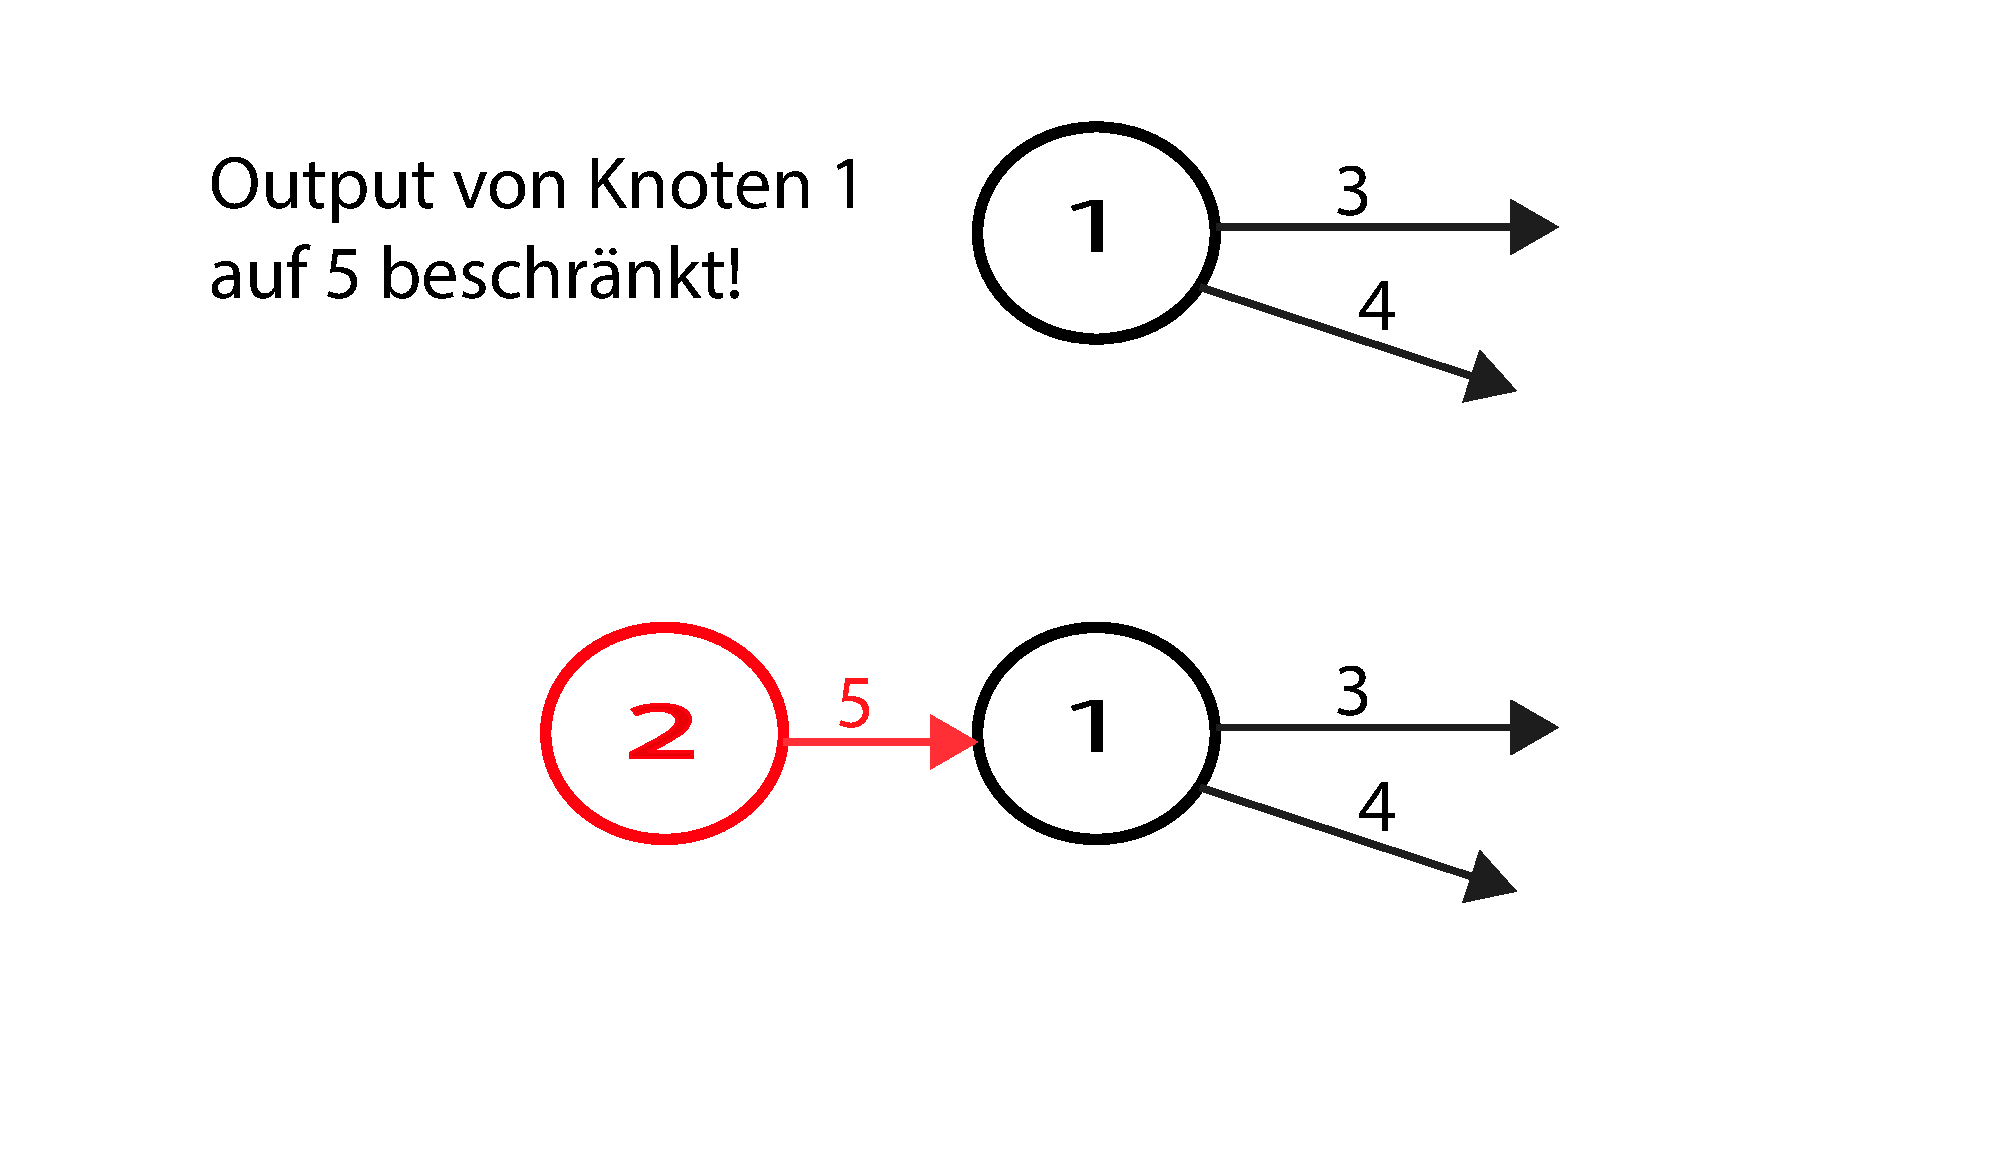
\includegraphics[width=\textwidth]{Content/Graphen/Constrain.pdf}
\end{minipage}

\begin{minipage}{0.33\textwidth}
	\textbf{Logistik-Problem} (Übung II.5/2):\\
	
	Lieferanten 0, 1, 2 haben eine Angebotskapazität\\
	Bezüger 3, 4, 5 haben eine Nachfrage\\
	neu eingefügte Quelle $s$ und Senke $t$ versorgen die Anbieter bzw. Bezüger mit den Angebot- bzw. Nachfragekapazitäten
\end{minipage}
\begin{minipage}{0.33\textwidth}
	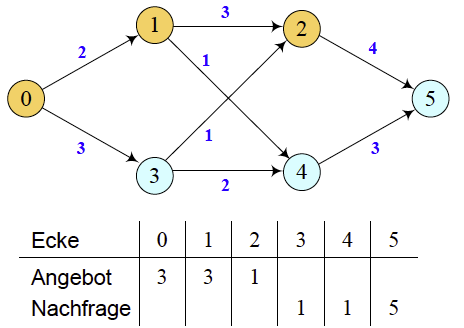
\includegraphics[width=\textwidth]{Content/Graphen/LogProb1.png}
\end{minipage}
\begin{minipage}{0.33\textwidth}	
	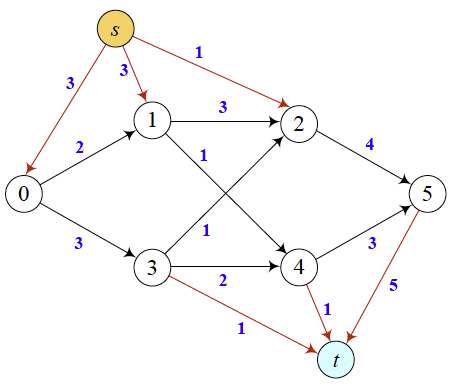
\includegraphics[width=\textwidth]{Content/Graphen/LogProb2.png}
\end{minipage}




% Maxflow Problem
\subsection{Maxflow Problem}

    Gesucht wird der maximal mögliche Fluss zwischen einer Quelle $s$ zu einer Senke $t$ ($st$-Netzwerk). Für Komplexität: $m$ = Anzahl Kanten, $f$ = maximaler Fluss von $s$ nach $t$.
    
    \begin{tabularx}{\textwidth}{p{3cm} X r}
      \textbf{Algorithmus} & \textbf{Beschreibung} & \textbf{Compl.}\\
      \hline
      \textbf{Ford-Fulkerson} \skript{22}
        & Kapazitäten müssen ganzzahlig sein! Pfade werden ausprobiert und jeweils der maximale Fluss durch diesen Pfad als (fiktiven) Rückwärtsfluss auf allen Kanten aufgetragen.
        & $O(m \cdot f)$\\
      \hline
      \textbf{Edmonds-Karp} \skript{24}
        & Gleich wie Ford-Fulkerson, aber es wird eine Breitensuche BFS angewendet.
        & $O(n\cdot m^2)$\\
      \hline
      \textbf{Max-Flow Min-Cut}
        & Der maximale Fluss in einem $st$-Netzwerk ist gleich dem minimalen Fluss über alle möglichen $st$-Schnitte.
        & -\\
      \hline
    \end{tabularx}


\subsubsection{Augmenting-Path Methode}

\begin{minipage}{0.7\textwidth}
	\begin{enumerate}
		\item Beliebigen Pfad von $s$ nach $t$ wählen
		\item Begrenzenden Teil-Pfad ermitteln; Kleinste Kapazität $f_i$ notieren
		\item Abziehen von $f_i$ von den Kapazitäten des gewählten Pfades $f_j$ ($f_j-f_i$)
		\item Wenn ein weiterer Pfad von $s$ nacht $t$ führt gehe zu  Punkt 1, andernfalls zu 5
		\item Der Gesamtfluss ist die Summe aller begrenzten Flüsse $f_{tot} = \sum_{i=1} f_i$
	\end{enumerate}
\end{minipage}
\begin{minipage}{0.3\textwidth}
	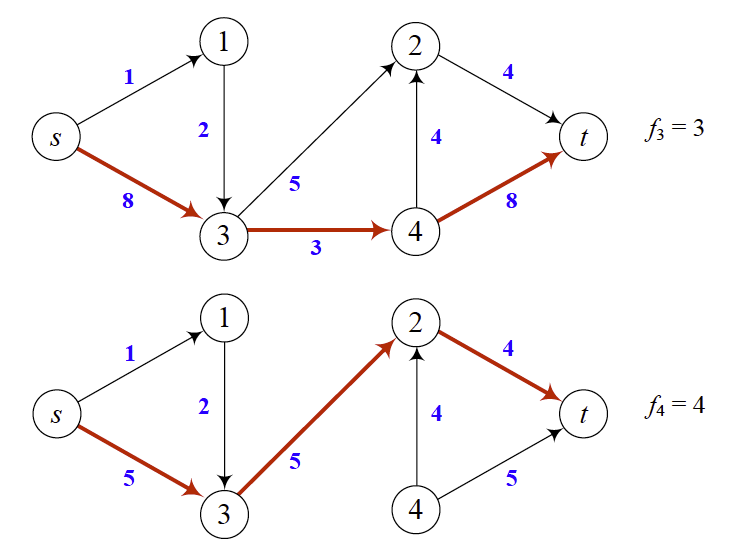
\includegraphics[width=\textwidth]{Content/Graphen/augmentingPathMethode.png}
\end{minipage}


Vorgehen ist problematisch, da es nicht möglich ist, einmal gewählte Flüsse wieder abzuwählen. (Greedy Verhalten)


\subsubsection{Ford-Fulkerson}
\begin{minipage}{0.7\textwidth}
Vorwärtspfad: Gibt an, um wieviel der Durchfluss erhöht werden kann.\\
Rückwärtspfad: Gibt an, um wieviel der Durchfluss verringert werden kann.
	\begin{enumerate}
		\item Beliebigen Pfad von $s$ nach $t$ wählen
		\item Begrenzenden Teil-Pfad ermitteln; Kleinste Kapazität $f_i$ notieren
		\item Abziehen von $f_i$ von den Vorwärtskanten $f_j$ und hinzufügen bei den Rückwärtskanten $r_j$ des gewählten Pfades $f_j$, Existiert keine Rückwärtskante muss diese eingefügt werden\\ ($f_j-f_i$ und $r_j + f_i$)
		\item Wenn ein weiterer Pfad von $s$ nach $t$ führt gehe zu  Punkt 1, andernfalls zu 5
		\item Der Gesamtfluss ist die Summe aller begrenzenden Flüsse $f_{tot} = \sum_{i=1} f_i$
	\end{enumerate}
\end{minipage}
\begin{minipage}{0.3\textwidth}
	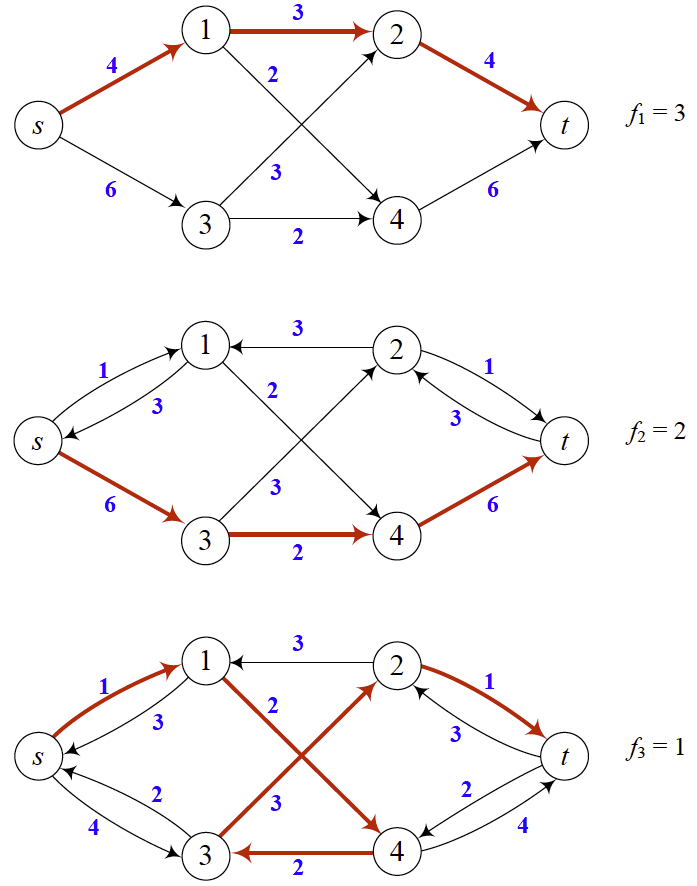
\includegraphics[width=\textwidth]{Content/Graphen/FordFulkerson.png}
\end{minipage}



\subsubsection{Max-Flow Min-Cut}
\textbf{Theorem:} \boxed{\text{Max-Flow ist gleich dem minimalen Fluss über alle möglichen ST-Cuts!}}

\begin{minipage}{0.6\textwidth}
	\textbf{Source Sink Cuts (ST-Cuts):}\\
	
	ST-Cut: Aufteilen der Ecken in eine Menge S (enthält Quelle s) und eine Menge T (enthält Senke t); $2^{|E|}$ Möglichkeiten\\
	
	Flow über ST-Cut: Summer aller Kapazitäten der Kanten, welche in S beginnen und in T enden!\\
	
	Max-Flow Min-Cut: im Bsp. ist der minimale Fluss über alle Cuts (Cut 5) gleich 7, was dem Maximalen Fluss des ST-Netzwerks entspricht.\\
	
\end{minipage}
\begin{minipage}{0.4\textwidth}
	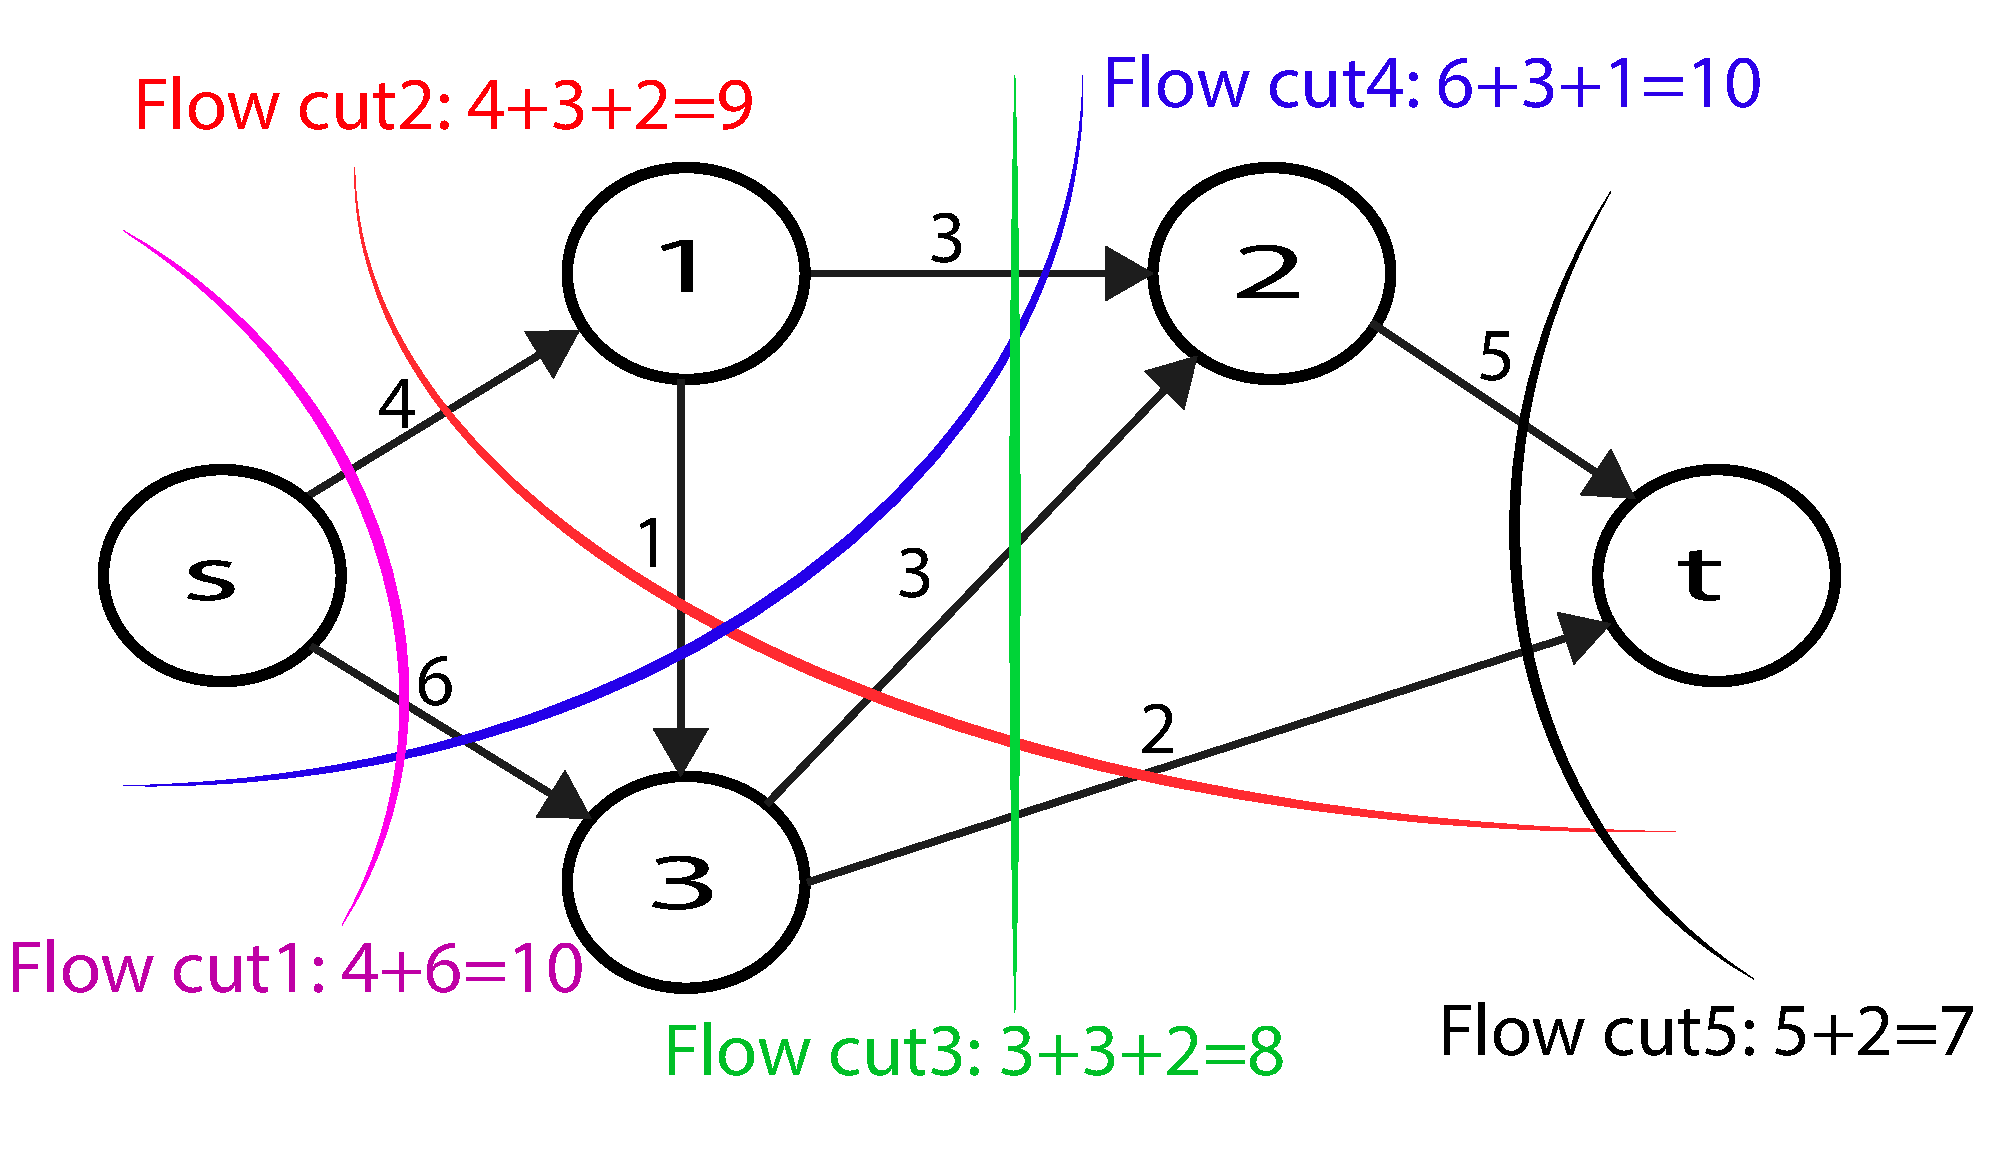
\includegraphics[width=\textwidth]{Content/Graphen/StCuts.pdf}
\end{minipage}
Min-Cut entspricht dem Nadelöhr, Max-Flow kann nur so viel sein, wie durchs Nadelöhr passt. 

% Maxflow Mincost
\subsection{Maxflow Mincost \skript{28}}
Die Lösung des Max Flow Problems ist nicht eindeutig, darum können weitere Kriterien hinzugefügt werden.\\

\textbf{Tipps:}
\begin{itemize}
\item Grosse Kreise zeichnen, damit Pfeilrichtungen eindeutig erkennbar.
\item Zweige mit geringen Transportkosten zuerst invertieren, um mit grosser Wahrscheinlichkeit negative Kreise zu unterbinden.
\end{itemize} 

\textbf{Vorgehen:}
\begin{enumerate}
	\item Ford-Fulkerson anwenden ($f_{tot}$ bleibt konstant!)
	\item Restnetzwerk durch Kantenkosten $k$ erweitern (Vorwärtskante: $+k$, Rückwärtskante: $-k$)
	\item Wenn Kreis mit negativen Kosten vorhanden gehe zu 4, andernfalls zu 5
	\item Fluss des neg. Kreises um die min. Kantenkapazität $c_{min}$ erhöhen (in Gegenrichtung!), gehe zu 3
	\item Gesamtfluss (max): $f_{tot}$ aus Ford-Fulkerson
	\item Gesamtkosten (min): Summe aller Rückwärtskantenkosten (RK) multipliziert mit der entsprechenden Kantenkapazität:\\  
	$k_{tot} = \sum\limits_{ i \in \text{alle RK}} c_i \cdot |k_i| $
\end{enumerate}

\textbf{Bsp.:}

\begin{minipage}{0.33\textwidth}
	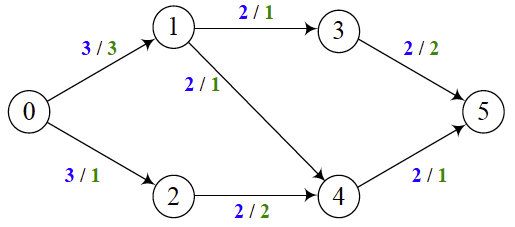
\includegraphics[width=\textwidth]{Content/Graphen/MaxFlowMinCost1.png}
	
	Ausgangsnetzwerk mit Kapazitäten\\ und Kosten
\end{minipage}
\begin{minipage}{0.33\textwidth}
	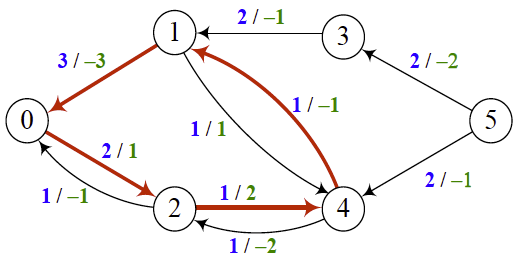
\includegraphics[width=\textwidth]{Content/Graphen/MaxFlowMinCost2.png}
	
	Restnetzwerk mit $f_{tot}=4$, $k_{tot}=21$,\\ Kreis mit neg. Kosten (rot,\\ $1+2-1-3 = -1$) mit min. Kantenkapazität $c_{min} = 1$
\end{minipage}
\begin{minipage}{0.33\textwidth}
	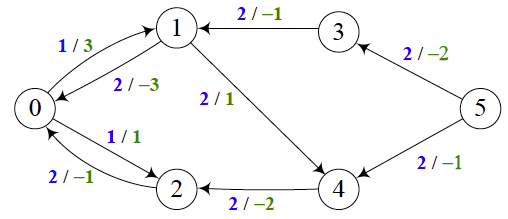
\includegraphics[width=\textwidth]{Content/Graphen/MaxFlowMinCost3.png}
	
	Neg.Kreis mit $c_{min}$ in Gegenrichtung erhöht\\
	$f_{tot} = 4$, 
	Gesamtkosten (RK!):\\ $k_{tot} = c_{1,s}\cdot|k_{1,s}| + c{2,1}\cdot|k_{2,1}|+... =\underbrace{2}_{c}\cdot\underbrace{(3+1+2+1+2+1)}_{\sum |k_i|}=20$
\end{minipage}

